%% LyX 2.1.4 created this file.  For more info, see http://www.lyx.org/.
%% Do not edit unless you really know what you are doing.
\documentclass[10pt,english]{article}
\usepackage[T1]{fontenc}
\usepackage[latin9]{inputenc}
\usepackage{geometry}
\geometry{verbose,tmargin=2cm,bmargin=2cm,lmargin=2cm,rmargin=2cm}
\usepackage{color}
\usepackage{babel}
\usepackage{float}
\usepackage{amsmath}
\usepackage{amssymb}
\usepackage{graphicx}
\usepackage{esint}
\usepackage[unicode=true,
 bookmarks=true,bookmarksnumbered=true,bookmarksopen=false,
 breaklinks=false,pdfborder={0 0 0},backref=false,colorlinks=true]
 {hyperref}

\makeatletter
%%%%%%%%%%%%%%%%%%%%%%%%%%%%%% User specified LaTeX commands.
\renewcommand\[{\begin{equation}}
\renewcommand\]{\end{equation}}

\makeatother

\begin{document}

\title{Adding Sensitivity to 21cm Inteferometric Probes of Reionization}

\maketitle

\section{Introduction}

The epoch of reionization represents the last key stage of the universe's
early evolution. Specifically, study of this event marks the intersection
of early cosmology and astrophysics. Understanding this event is important
not only as a scientific goal of its own, but also potentially provides
crucial information to fundamental nature of inflation, neutrino mass
and phenonmenology of the first stars and galaxies alike. 

Arguably the most promising observational probe of the epoch of reionization
comes from measurement of the ``spin-flip'' transition of neutral
hydrogen of characteristic wavelength 21cm. While probes relying on
emission and scattering of free electrons are limited to the lower
redshifts after the completion of reionization, the 21cm line directly
probes the abundance and distribution of neutral hydrogen, and thus
would potentially shed light on the entire cosmic dawn. Thus radio
interferometry techniques to measure the 21cm power spectrum has been
a top priority in astronomy. Cuurrent generation instruments include
the Precision Array for Probing the Epoch of Reionization (PAPER),
Murchison Widefield Array (MWA), Low Frequency Array (LOFAR), and
next generation instruments such as the Hydrogen Epoch of Reionization
Array (HERA) and the Square Kilometer Array Low (SKA low) are under
construction. 

One of the main challenges of interferometric observations of cosmic
21cm line is the foreground contaminations. Both sources within our
galaxy, and to a lesser extent sources outside of our galaxy emit
radio contaminations up to five orders of magnitude higher than the
reionization signal. There are two common methods to deal with the
foreground contamination. In the first, individual sources are identified
and removed, sometimes called the foreground removal technique. The
other technique, commonly refered to as foreground avoidance, makes
use of the fact that most foreground contamination is a smooth spectrum,
and thus is contrained to a Fourier domain ``foreground wedge''.
The main challenge of using the latter technique is the sensitivity,
or the signal to noise ratio. This is the motivation for the design
of the maximum redundancy arrays such as MWA, PAPER, and HERA. While
traditional imaging arrays such as the Very Large Array (VLA) focus
on Fourier mode uv coverage, the redundant arrays have many tightly
packed antennas at equal spacing. Since baselines of the same length
and orientation measure the same Fourier modes on the sky, the maximum
redundancy arrays is able to increase the signal to noise ratio of
the Fourier mode in question. Ali2015 provided the newest upper limit
to the power spectrum measurements with the PAPER-64 data. Some models
expect that the sensitivity required for detection is a factor of
2 away. 

The earth's rotation causes the baseline to sweep through different
areas of the sky during the day. This effect is used extensively to
improve uv coverage in imaging with minimum redundancy arrays. In
a redundant array, baselines that are slightly different rotate into
each other at a time delay. Here we present a method to improve the
sensitivity of the maximum redundancy arrays by considering the uv
redundancy of different baselines at a time lag. In section 2 we present
the basic search algorithm for this time delay. In section 3 we present
a necessary correction and comparison with simulated data. 


\section{Time delayed redundancy}

Baselines of the same length and orientation are traditionally called
``redundant baselines'', because they measure the same Fourier mode
in the sky. In order to eliminate confusion, we shall introduce slightly
different terminology. We'll call baselines that are the same length
and orientation ``equivalent baselines''. Two equivalent baselines
will be redundant with each other simultaneously. Some non-equivalent
baselines can also be redundant if their respected time series is
shifted with respect to one another by a certain delay. We call the
latter ``near equivalent baselines''. It is our goal to a) identify
the near equivalent baselines that give good delayed redundancy, b)
to find this delay for a given pair of baselines, and c) to quantify
the sensitivity improvement associated with cross multiplying such
a pair of nonequivalent baselines. 


\subsection{Cross multiplication of near redundant data}

To begin, we first derive theoretical expectations of cross correlation
of two near-equivalent baselines. Given a point source on the sky,
each baseline measures a track of the source in uv plane. We identify
redundancy of near equivalent baselines for that point source as crossings
of the tracks. Since processed data are measured at discrete time
intervals (in lst-binned PAPER-64 data it's 42.9 seconds ), we do
not have exact overlap of two data points in uv space. We thus need
to find a way to cross multiply data points that are separated by
a short distance in uv space and recover the power spectrum. 

We take the visibility as 
\[
\begin{aligned}V_{\nu}(b) & =\int d\Omega A(\hat{r})I(\hat{r})\exp\left[-2\pi i\frac{\nu}{c}b\cdot\hat{r}\right],\\
 & \approx\frac{2k_{B}}{\lambda^{2}}\int d\Omega A(\hat{r})T(\hat{r})\exp\left[-2\pi i\frac{\nu}{c}b\cdot\hat{r}\right],\\
 & =\frac{2k_{B}}{\lambda^{2}}\int\frac{d^{3}r}{X^{2}Y}A(r)T(r)e^{-ikr}.
\end{aligned}
\]
Here $\lambda$ is a mean wavelength, $\boldsymbol{b}$ is the baseline
length, $\hat{\boldsymbol{r}}$ is a direction in the sky, $A$ is
the beam, and $I$ is the intensity, which has been related to $T$,
the brightness temperature. In the last line $(r_{x},r_{y},r_{z})=(Xl,Xm,Y\nu)$,
and $(Xk_{x},Xk_{y},Yk_{z})=2\pi(u,v,\eta)$. 

We define the delay transformed visibility:
\[
\begin{aligned}V(b) & =\int d\nu V_{\nu}(b)\exp\left[-2\pi i\nu\eta\right],\\
 & =\frac{2k_{B}}{\lambda^{2}}\int d\Omega d\nu A(\hat{r},\nu)T(\hat{r},\nu)\exp\left[-2\pi i\left(\frac{\nu}{c}b\cdot\hat{r}+\nu\eta\right)\right]
\end{aligned}
\]


We'd like to relate this to the 3 dimensional power spectrum. We start
by noting that 
\[
\begin{aligned}r & =\frac{c}{H_{0}}\int_{0}^{z}\frac{dz'}{E(z')}-\frac{c(1+z)^{2}}{\nu_{21}H_{0}E(z)}\left(\nu-\nu_{21}\right),\\
 & \equiv D_{c}-Y\Delta\nu,
\end{aligned}
\]
where $\nu_{21}=1420MHz$ is the 21cm transition rest frequency, and
\[
E(z)=\sqrt{\Omega_{m}(1+z)^{3}+\Omega_{\Lambda}}.
\]
So
\[
\nu=\frac{D_{c}-r}{Y}+\nu_{21}.
\]
Thus $d\nu=-dr/Y$ and we can rewrite the delayed transformed visibility
as 
\[
\begin{aligned}V(b) & =\frac{1}{Y}\int_{H}d^{3}rA(r)I(r)\exp\left[2\pi i\frac{r}{Y}\left(\frac{b\cdot\hat{r}}{c}+\eta\right)\right]\exp\left[-2\pi i\left(\frac{b}{c}\cdot\hat{r}+\eta\right)\left(\frac{D_{c}}{Y}+\nu_{21}\right)\right]\end{aligned}
.
\]
$A$ is a patch of shell 

The beam reception pattern $A$ is dimensionless, normalized to 1
at its peak (zenith), and we assume it to be the same for all baselines.
We introduce the Fourier temperature and window function

\[
\begin{aligned}\tilde{T}(k) & =\int\frac{d^{3}r}{X^{2}Y}T(r)e^{-ikr},\\
W(k) & =\int d^{3}rA(r)e^{-ikr}.
\end{aligned}
\]
Here 
\[
k=2\pi\frac{b}{cY}.
\]
By the convolution theorem, we have
\[
\begin{aligned}\tilde{V}(k) & =\frac{2k_{B}}{\lambda^{2}}\int\frac{d^{3}r}{Y}A(r)T(r)e^{-ikr},\\
 & =\frac{2k_{B}}{\lambda^{2}}\frac{1}{(2\pi)^{3}}\int d^{3}k_{1}W(k_{1})\tilde{T}(k+k_{1}).
\end{aligned}
\]
With a time offset, the sky has moved from coordinates $r$ to $\Gamma r$.
With implicit bounds of integrals from $-\infty$ to $\infty$, we
have

\[
\begin{aligned}\langle V^{*}(k)V(k')\rangle & =\left(\frac{2k_{B}}{X^{2}Y\lambda^{2}}\right)^{2}\int d^{3}rd^{3}r'\left(\langle T^{*}(r)T(\Gamma r')\rangle\right)A^{*}(r)A(r')\Phi(b,\eta),\\
 & =\left(\frac{2k_{B}}{X^{2}Y\lambda^{2}}\right)^{2}\int d^{3}rd^{3}r'\left(\int\frac{d^{3}\kappa}{(2\pi)^{3}}\frac{d^{3}\kappa'}{(2\pi)^{3}}\langle T^{*}(\kappa)T(\kappa')\rangle e^{-i(\kappa r-\kappa'\Gamma r')}\right)A^{*}(r)A(r')\Phi(b,\eta),\\
 & =\left(\frac{2k_{B}}{X^{2}Y\lambda^{2}}\right)^{2}\int d^{3}rd^{3}r'\left(\int\frac{d^{3}\kappa}{(2\pi)^{3}}P(\kappa)e^{-i\kappa(r-\Gamma r')}\right)A^{*}(r)A(r')\Phi(b,\eta),\\
 & =\left(\frac{2k_{B}}{X^{2}Y\lambda^{2}}\right)^{2}\int d^{3}rd^{3}r'\xi(r-\Gamma r')A^{*}(r)A(r')\Phi(b,\eta),\\
 & \approx\left(\frac{2k_{B}}{X^{2}Y\lambda^{2}}\right)^{2}P(k)\int d^{3}rd^{3}r'\delta_{D}^{(3)}(r-\Gamma r')A^{*}(r)A(r')\exp\left[-i\frac{2\pi}{c}\left(b\cdot\nu\hat{r}-b'\cdot\nu'\hat{r'}\right)\right]\exp\left[-i2\pi\eta\left(\nu\hat{r}-\nu'\hat{r'}\right)\right],\\
 & =\left(\frac{2k_{B}}{X^{2}Y\lambda^{2}}\right)^{2}P(k)\int d^{3}r|A^{*}(r)A(\Gamma r)|\exp\left[-i2\pi\nu_{r}\left\{ \hat{r}\cdot(\frac{b}{c}+\eta c\hat{r})-\hat{\Gamma r}\cdot(\frac{b'}{c}+\eta'\hat{\Gamma r})\right\} \right],
\end{aligned}
\]
where the phase term is 
\[
\Phi(b,\eta)=\text{\ensuremath{\exp\left[-i\frac{2\pi}{c}\left(b\cdot\nu\hat{r}-b'\cdot\nu'\hat{r'}\right)\right]\exp\left[-i2\pi\eta\left(\nu\hat{r}-\nu'\hat{r'}\right)\right]},}
\]
The first to second line follows from assumption of Gaussian random
sky, and the second to third line follows from the assumption that
the 3D power spectrum varies neglegibly over the region of interest
so that $\hat{P_{21}}(k+k_{2})\approx\hat{P_{21}}(k)$. In the last
line we have written $\nu_{r}$ to remind us that $\nu$ and $r$
are related by Eq. 4. Since $\Gamma$ is a sky rotation, it doesn't
affect $\nu$, hence we have taken $\nu_{r}$ outside the parenthesis.
Notice also that we have omitted a phase factor $ $ because it would
drop out in the last step. 

Now plugging in result from Eq. 4, we see 

\[
\boxed{\langle V^{*}(k)V(k')\rangle=P(k)\left(\frac{2k_{B}}{X^{2}Y\lambda^{2}}\right)^{2}\Psi\int d^{3}r|A^{*}(r)A(\Gamma r)|\exp\left[i\frac{2\pi}{cY}\vec{r}\cdot\left(b-b'\right)\right],}
\]
where $\Psi=\exp\left[-2\pi i\frac{b-b'}{c}\cdot\hat{r}\left(\frac{D_{c}}{Y}+\nu_{21}\right)\right]$
is a phase that's fixed.  So in conclusion the cross correlation of
visibilities seperated by $\Delta u$ apart in uv space is proportional
to the power spectrum times the Fourier transform of the cross multiplied
beam pattern. One can then in principle combine information from different
baseline pairs if one corrects for the phase and normalization. 

\begin{figure}[H]
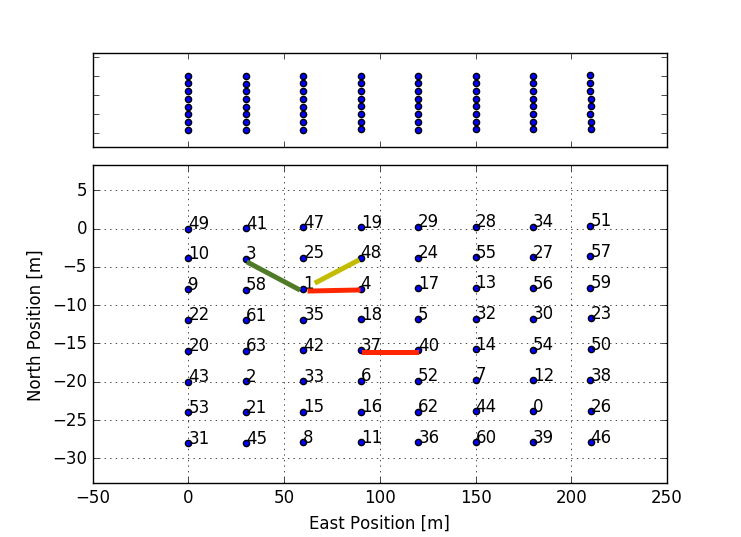
\includegraphics[scale=0.5]{64layout}

\caption{The PAPER 64 layout. Top panel shows the antenna positions drawn to
scale, bottom panel show the antenna labels and distances. }
\end{figure}


We shall use the 64-antenna PAPER array to demonstrate. The PAPER
64 array is located in the Karoo desert in South Africa (30:43:17.5
S, 21:25:41.8 E). The layout pattern with antenna labels are show
in Fig. 1. I show denote a baseline with the antconfigWe see the antenna
spacing in North-South directions are comparatively close (4m), so
that baselines such as 0\_44 and 0\_7 are very close to equivalent. 


\section{Technique}

For a given point source in the sky, each baseline at a particular
instant corresponds to a point in UV space. Thus as the earth rotates,
the point source traces out a track in UV plane for a given baseline.
As an example, we show the rotation tracks for a source that passes
through zenith in Fig. \ref{fig:Tracks-of-PAPER64} below for the
baselines of PAPER 64:

\begin{figure}[H]
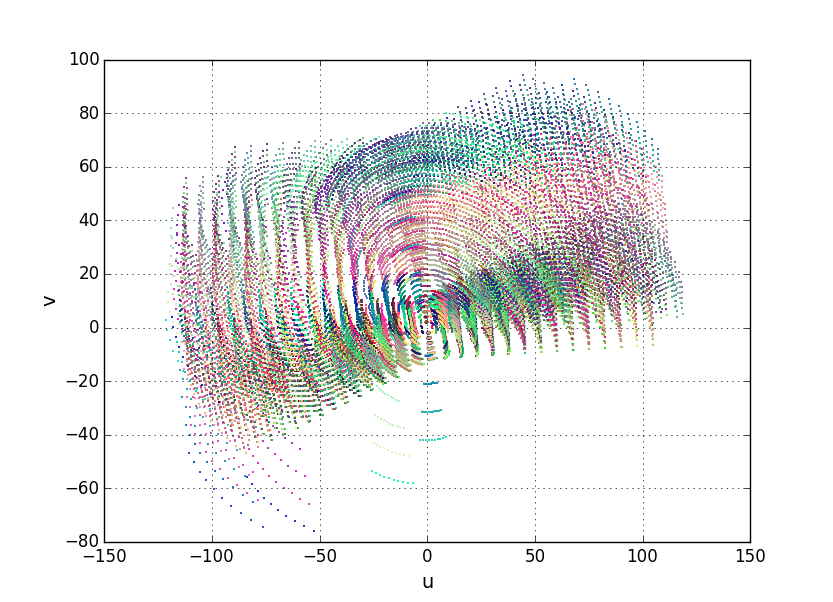
\includegraphics[scale=0.5]{tracks}

\caption{Tracks of PAPER64 for a hypothetical source that passes through zenith.
Color scale simply represents different tracks. Spacing between dots
are characteristic of time resolution of compressed data. As the earth
rotates, tracks are traced out counterclockwise. \label{fig:Tracks-of-PAPER64}}
\end{figure}


The beam squared and its Fourier transform are given as

\begin{figure}[H]
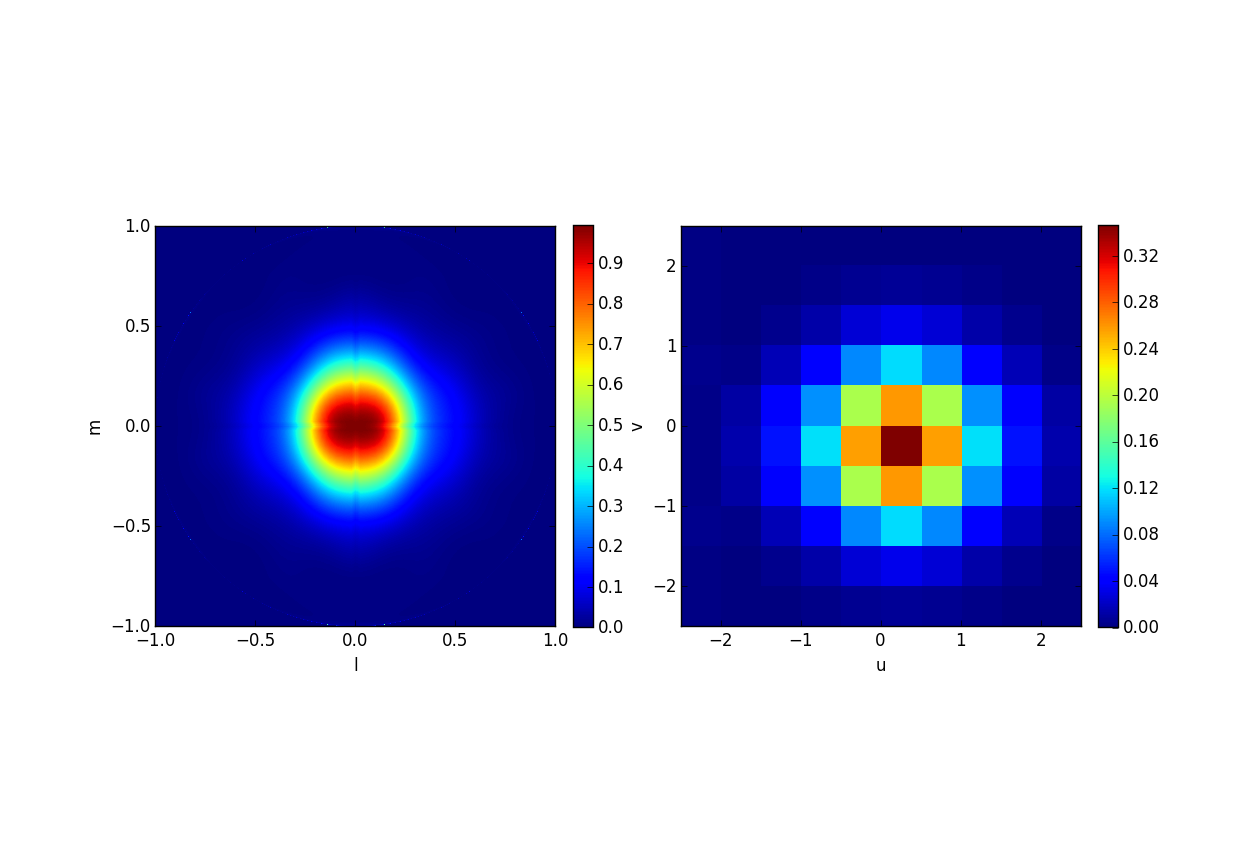
\includegraphics[scale=0.4]{64beam}

\caption{The PAPER 64 layout. Top panel shows the antenna positions drawn to
scale, bottom panel show the antenna labels and distances. }
\end{figure}


In practice, we first implement a search algorithm that grids the
uv plane and search for intersections, then confirm the time delay
by plotting a) cross correlated visibilities from simulated random
sky, and b) theoretical proportion factor $\int d^{3}r|A^{*}(r)A(\Gamma r)|\exp\left[-i\frac{2\pi}{c}\nu\hat{r}\cdot\left(b-b'\right)\right]$
from Eq. 10. 


\subsection{Grid search algorithm}

The gridding algorithm sets up grids on the UV-plane, creates a point
source that passes through zenith, and searches for intersections
of the UV tracks. The search compares each track to each other track
to locate the closest approaches. To optimize performance, the algorithm
first sets up coarse grids, locate the cells that contain data points
from more than one tracks, then fine grains the cell to determine
the point of closest approach. Fig {[}insert{]} illustrates this procedure.
This algorithm is mainly used to determine which baselines to cross
correlate, and give a rough estimate of the time offset. We indeed
find that baselines 0\_44 and 0\_7 give the closest approach wiht
a time offset of roughly 0.03 sidereal days. In reality, a wide beam
(e.g. Fig. 2) samples a patch of sky, not just a point source. And
thus the real UV representation of a baseline is the track convolved
with an appropriate point spread function. Accounting for these factors
accurately in this context is difficult. Thus for accurate determination
of the time offset, we resort to two other methods. It is also worth
pointing out that the near-redundant pairs is not only useful at a
particular time corresponding to the crossing. The search algorithm
uses a fiducial point source in the sky to find the offset, and all
time-stamps separated by this offset corresponds to UV-track crossing
of a point in the sky, and thus all data of the two baselines can
be utilized. 


\subsection{Gaussian sky simulation}

Having found the pairs of baselines to cross-correlate, and a rough
estimate of the time offset, we make a more accurate determination
of the time offset. Here we take N random realizations of the sky
on a healpix map\footnote{We use functionalities in the python package AIPY for healpix mapping
as well as coordinate transforms. }. For each realization, each pixel is given a Gaussian random value
of brightness temperature. We then rotate the baseline positions by
a simple rotation matrix, recording the visibilities, for each baseline,
as given in Eq. 1 \footnote{As a caveat, there are two obvious ways to achieve the rotation. One
can either fix the sky and rotate the baselines, or the other way
around. We found however, that we must not physically rotate the sky
map, for the numerical roundoffs due to finite resolutions of the
map turns out to be significant. Thus we let the sky, represented
by the healpix map, be fixed, and rotate the baselines. }. The resulting visibilities for the two baselines are then convolved
via the Fourier convolution theorem, to obtain values of the cross
correlation as a function of time-offset. The peak of the curve then
corresponds to maximum redundancy. The accuracy of this result is
limited by (simulated) cosmic variance and finite spacial resolution,
and hence can be beat down by averaging over a large number of universes.
A numerical estimate of the error of the peak height with $N=1$ is
$\lesssim20\%$, and thus with $N=2500,$ we achieve an error of peak
height $<0.5\%$. An example is shown in Fig. {[}insert{]} 


\subsection{Theoretical determination}

To test our understanding of the time-offset, and to verify our derivation
in Eq. 10 makes sense, we must check the curve obtained in Fig. against
one from the multiplicative factor in Eq. 10. In particular, we'd
really like to compare the peak location as well as height. For the
latter, the most useful information comes in its comparison with that
of an equivalent baseline. Thus in Fig. {[}insert{]} below we show
on the left comparison of the convolution of an equivalent baseline,
normalized to 1 at the peak, whose location is at 0 offset as expected.
On the right we show comparison of the baseline pair found in the
grid search. The peaks are normalized with the same factor as the
peak height on the left, i.e. the two plots have thus the same scale
on the vertical axis. The height of the plot on the right thus quantifies
the added sensitivity. 

\begin{figure}[H]
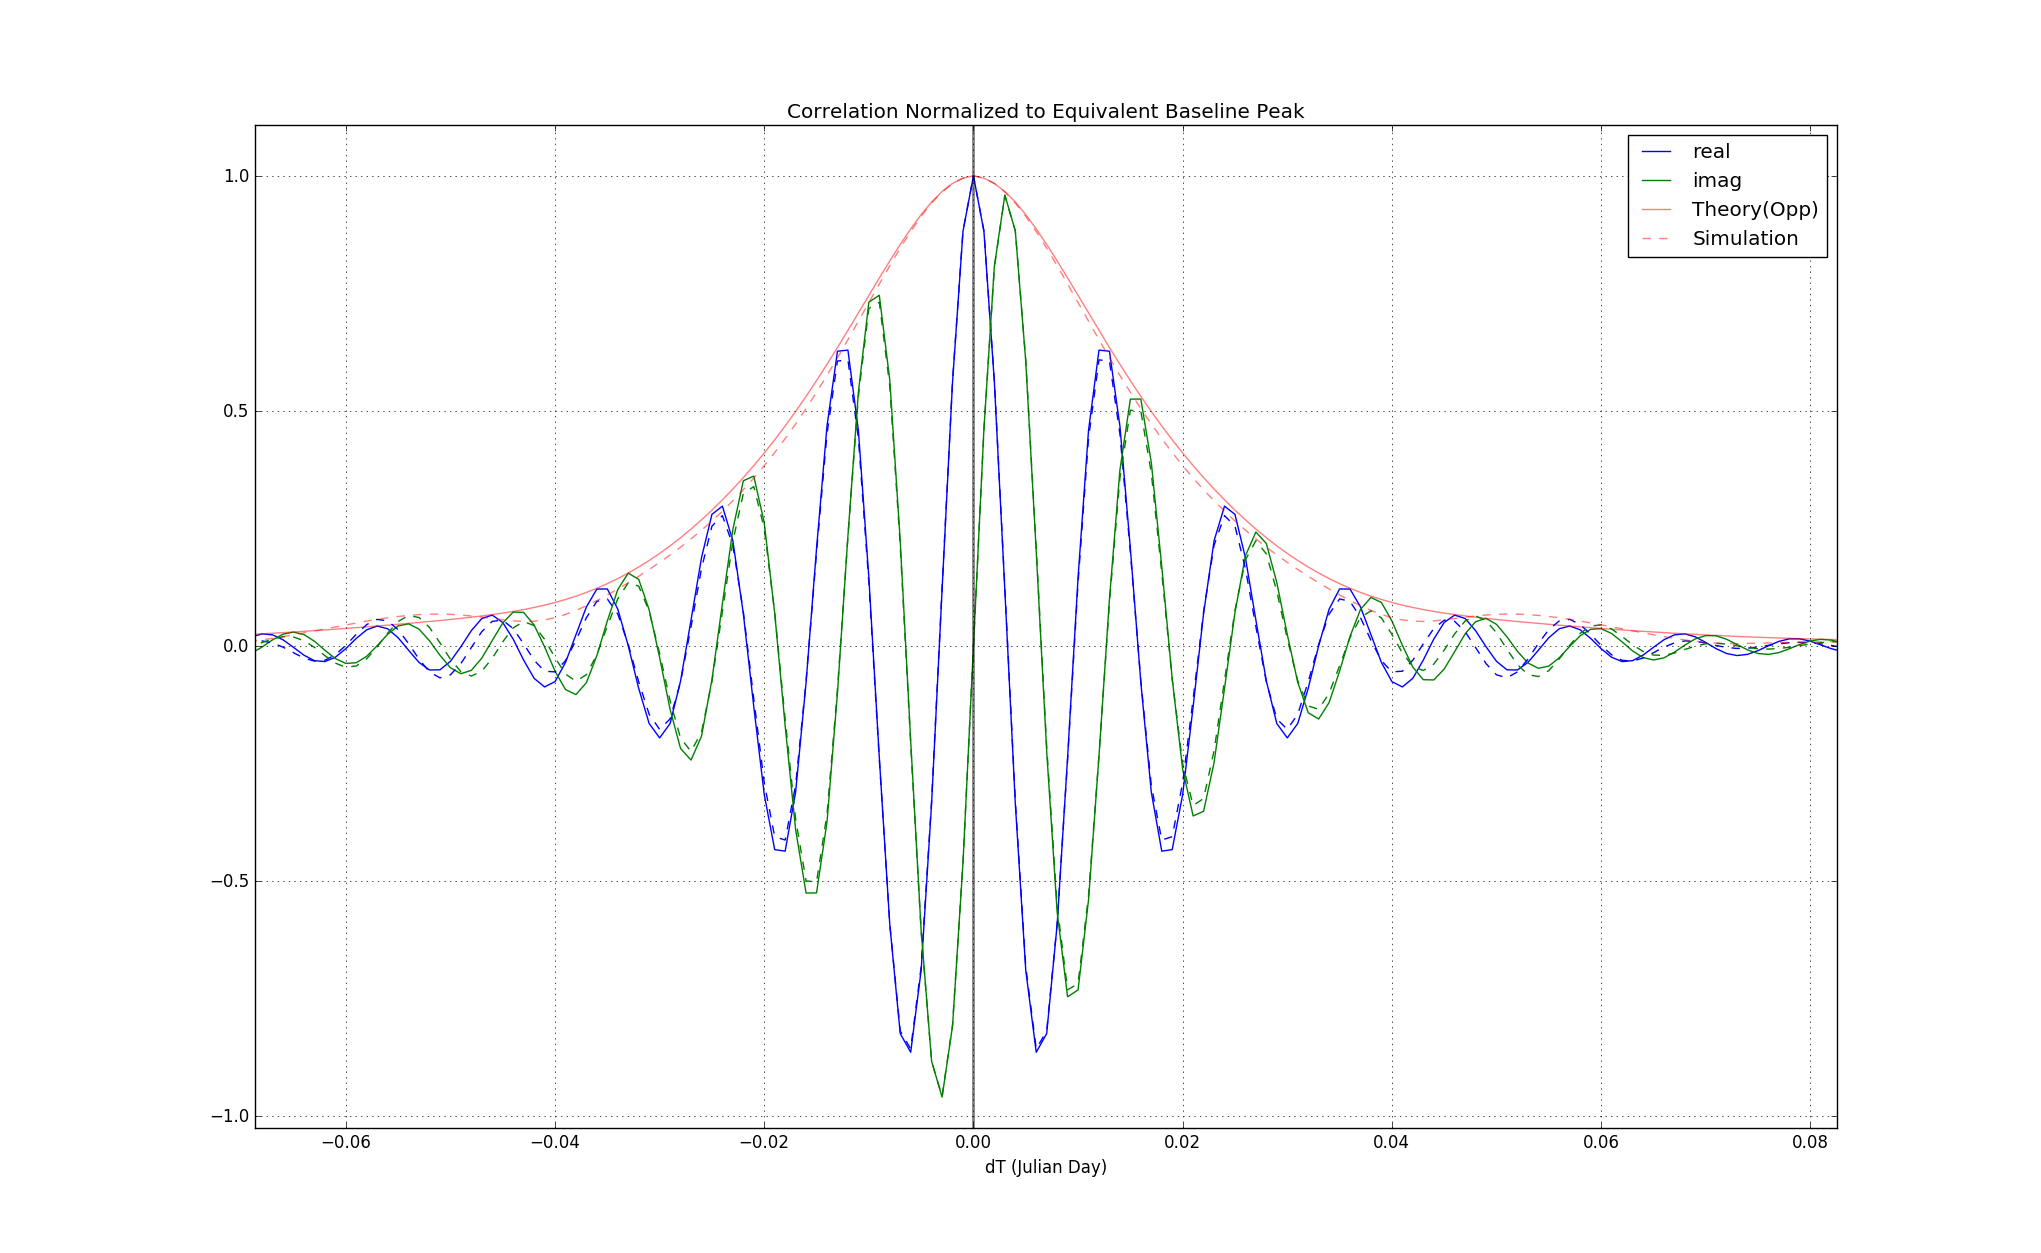
\includegraphics[scale=0.25]{redun_agree}

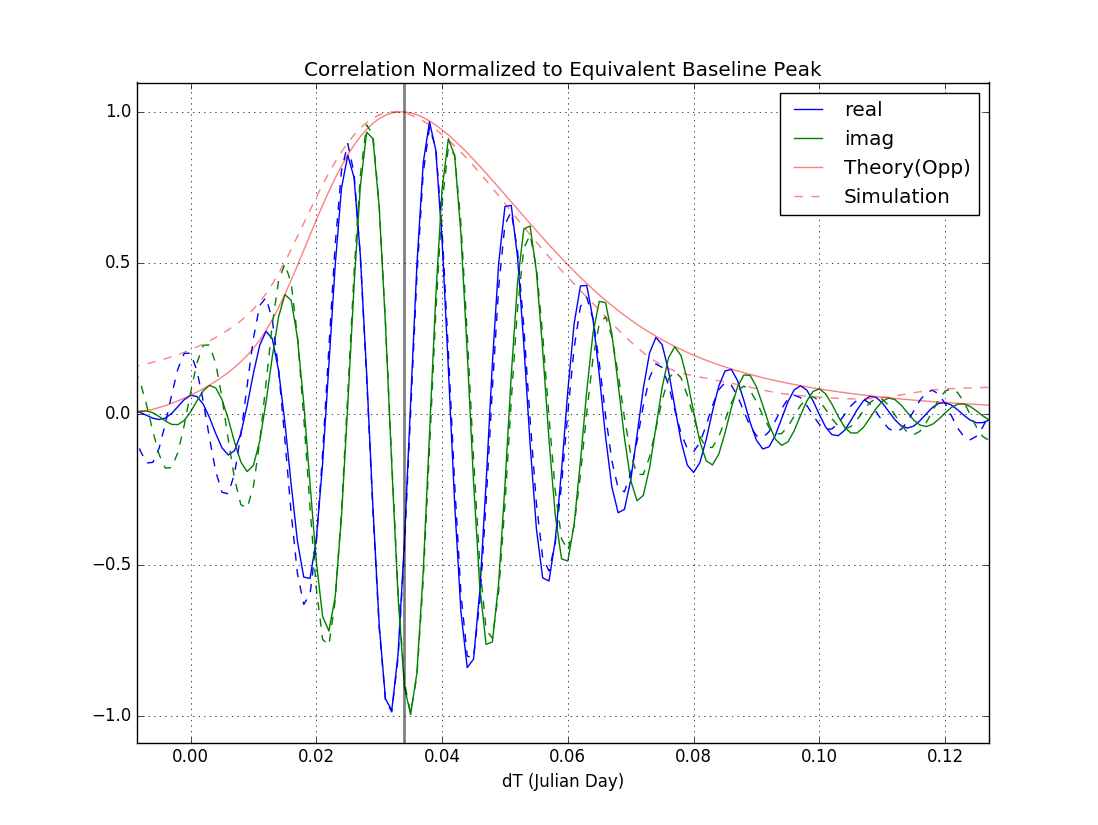
\includegraphics[scale=0.3]{simucorroff}

\caption{The PAPER 64 layout. Top panel shows the antenna positions drawn to
scale, bottom panel show the antenna labels and distances. }
\end{figure}



\section{Application to PAPER 64}


\subsection{Expected Sensitivity contribution}

The latest release of PAPER 64 data uses baselines sep-1,1, sep0,1
and sep1,1 {[}cite Ali2015{]}, and achieved a $2\sigma$ upper limit
of $22.4mK^{2}$. There, the three sets of equivalent baselines are
only cross multiplied by itself. Assuming that each baseline delivers
the same quality of data, the relative contribution to sensitivity
can be estimated 
\end{document}
